\documentclass[a4paper,10pt]{llncs}
\usepackage{fullpage}
\usepackage[british]{babel}
\usepackage[T1]{fontenc}
\usepackage{amsmath}
\usepackage{amssymb}
\usepackage[T1]{fontenc}
\usepackage[latin1]{inputenc} 
%\usepackage{amsthm} \newtheorem{theorem}{Theorem}
\usepackage{color}
\usepackage{float}



\usepackage{caption}
\DeclareCaptionFont{white}{\color{white}}
\DeclareCaptionFormat{listing}{\colorbox{gray}{\parbox{\textwidth}{#1#2#3}}}
\captionsetup[lstlisting]{format=listing,labelfont=white,textfont=white}


\usepackage{alltt}
\usepackage{listings}
 \usepackage{aeguill} 
\usepackage{dsfont}
%\usepackage{algorithm}
\usepackage[noend]{algorithm2e}
%\usepackage{algorithmicx}
\usepackage{subfig}
\lstset{% parameters for all code listings
	language=Python,
	frame=single,
	basicstyle=\small,  % nothing smaller than \footnotesize, please
	tabsize=2,
	numbers=left,
%	framexleftmargin=2em,  % extend frame to include line numbers
	%xrightmargin=2em,  % extra space to fit 79 characters
	breaklines=true,
	breakatwhitespace=true,
	prebreak={/},
	captionpos=b,
	columns=fullflexible,
	escapeinside={\#*}{\^^M}
}


% Alter some LaTeX defaults for better treatment of figures:
    % See p.105 of "TeX Unbound" for suggested values.
    % See pp. 199-200 of Lamport's "LaTeX" book for details.
    %   General parameters, for ALL pages:
    \renewcommand{\topfraction}{0.9}	% max fraction of floats at top
    \renewcommand{\bottomfraction}{0.8}	% max fraction of floats at bottom
    %   Parameters for TEXT pages (not float pages):
    \setcounter{topnumber}{2}
    \setcounter{bottomnumber}{2}
    \setcounter{totalnumber}{4}     % 2 may work better
    \setcounter{dbltopnumber}{2}    % for 2-column pages
    \renewcommand{\dbltopfraction}{0.9}	% fit big float above 2-col. text
    \renewcommand{\textfraction}{0.07}	% allow minimal text w. figs
    %   Parameters for FLOAT pages (not text pages):
    \renewcommand{\floatpagefraction}{0.7}	% require fuller float pages
	% N.B.: floatpagefraction MUST be less than topfraction !!
    \renewcommand{\dblfloatpagefraction}{0.7}	% require fuller float pages

	% remember to use [htp] or [htpb] for placement


\usepackage{fancyvrb}
%\DefineVerbatimEnvironment{code}{Verbatim}{fontsize=\small}
%\DefineVerbatimEnvironment{example}{Verbatim}{fontsize=\small}

\usepackage{url}
\urldef{\mailsa}\path|sharyari@gmail.com |    
\newcommand{\keywords}[1]{\par\addvspace\baselineskip
\noindent\keywordname\enspace\ignorespaces#1}


\usepackage{tikz} \usetikzlibrary{trees}
\usepackage{hyperref}  % should always be the last package

% useful colours (use sparingly!):
\newcommand{\blue}[1]{{\color{blue}#1}}
\newcommand{\green}[1]{{\color{green}#1}}
\newcommand{\red}[1]{{\color{red}#1}}

% useful wrappers for algorithmic/Python notation:
\newcommand{\length}[1]{\text{len}(#1)}
\newcommand{\twodots}{\mathinner{\ldotp\ldotp}}  % taken from clrscode3e.sty
\newcommand{\Oh}[1]{\mathcal{O}\left(#1\right)}

% useful (wrappers for) math symbols:
\newcommand{\Cardinality}[1]{\left\lvert#1\right\rvert}
%\newcommand{\Cardinality}[1]{\##1}
\newcommand{\Ceiling}[1]{\left\lceil#1\right\rceil}
\newcommand{\Floor}[1]{\left\lfloor#1\right\rfloor}
\newcommand{\Iff}{\Leftrightarrow}
\newcommand{\Implies}{\Rightarrow}
\newcommand{\Intersect}{\cap}
\newcommand{\Sequence}[1]{\left[#1\right]}
\newcommand{\Set}[1]{\left\{#1\right\}}
\newcommand{\SetComp}[2]{\Set{#1\SuchThat#2}}
\newcommand{\SuchThat}{\mid}
\newcommand{\Tuple}[1]{\langle#1\rangle}
\newcommand{\Union}{\cup}
\usetikzlibrary{positioning,shapes,shadows,arrows}

\pagestyle{empty}

\title{\textbf{Modelling the Suzuki-Kasami Algorithm\\ with the SPIN Model Checker}}

\author{Jonathan Sharyari}

\institute{Freie Universit{\"a}t Berlin, Computer Science Department\\
Takustra{\ss}e 9. 14195 Berlin, Germany\\
\mailsa
}
\begin{document}
\maketitle


\begin{abstract}
In 1985, Suzuki and Kasami presented two distributed algorithms for mutual exclusion. In this paper, the claim of mutual exclusion, deadlock and starvation freedom are tested using model checking techniques. Using the spin model checker, a counterexample to deadlock freedom was found for one of the algorithms, and a modification is proposed that guarantees deadlock freedom.
\end{abstract}


\section{Introduction}
Model checking is the process of automatically verifying the correctness of a system description with respect to its specifications, by examining a model corresponding to the system. The result of model checking with respect to some property is in general a certificate of correctness, or a trail that does not satisfy the property, i.e. a counterexample.

There are many tools for model checking available, with different approaches to model checking and with different strengths and weaknesses. The SPIN Model checker (typically written Spin) is a widely used tool for the model checking of distributed and concurrent systems.

The Spin model checker was used mainly while both the tested pseudo code and the spin modelling language (promela) has a syntax close to that of the C programming language, thus making it easier to ensure that the model in fact corresponds to the algorithm of interest.


\subsection{Suzuki and Kasami's Algorithm}

The Suzuki/Kasami algorithm\cite{Suzuki} (henceforth abbreviated \textsc{ska}), is a distributed mutual exclusion-algorithm that requires at most N message exchanges for every mutual exclusion invocation between N computer nodes.

Each of the N nodes between which mutual exclusion is to be realized runs two processes P1 and P2. Each node has two local arrays RN and LN and a queue Q, all of which are accessible by P1 and P2.

The array RN holds the latest received request identifier for each other node. Similarly, LN holds the request identifier of the latest carried out request of all the other nodes, of which the node has been notified. Since the algorithm is distributed, the local arrays RN and LN are not necessarily the same for each node; for each node they represent only the information of which the node has been notified.

The local queue Q holds the nodes that are currently requesting the privilege, in the order the requests have been received.

When a node $node_i$ wants to enter its critical section with its main process P1, it needs to have the privilege to do so. In case the node already holds the privilege, it enters the critical section directly, without informing the other processes and does \emph{not update the arrays RN and LN}. Otherwise a \texttt{REQUEST(i, n)} message is sent to all other nodes, where i is the nodes identifier (index) and n is the request identifier.

A requesting node must wait until it receives a \texttt{PRIVILEGE} message, before accessing its critical section. When it is done, it updates its queue by appending all the requesting nodes not currently in the queue. Then, a \texttt{PRIVILEGE} is sent to the node first in Q, and that node is removed from the queue.

In process P2 \texttt{REQUEST(i,n)} messages are received. The array RN is updated, so that the corresponding entry RN[i] is set to n. If the node currently holding the \texttt{PRIVILEGE} is not itself waiting for the privilege, it will forward the \texttt{PRIVILEGE} to $node_i$ by sending a \texttt{PRIVILEGE(Q, LN)} message.

The pseudo-code proposed in the original paper is listed in appendix \ref{sec:ska}.

\subsection{Suzuki and Kasami's Modified Algorithm}
The \textsc{ska} algorithm has the disadvantage of request identifier numbers being unbounded. In a modified version of the \textsc{ska} algorithm (henceforth abbreviated \textsc{skam}), Suzuki and Kasami propose slight changes to the above algorithm in order to bound the request identifiers by a value L but with the cost of additional message exchanges.

The \textsc{skam} algorithm introduces a third process P3 to each node, a new message type \texttt{REPLY} and an array \texttt{RequestCount[2]} local to process P2.

When a node $n_1$ receives a \texttt{REQUEST} message from another node $n_3$, it will increase the value of the local variable \texttt{RequestCount[2]} by one. If \texttt{RequestCount[2]} is equal to L, it is reset to zero and a \texttt{REPLY} message is sent back to the $n_3$ and RN[2] is set to 0.

The process P3 receives the \texttt{REPLY} messages and increments the variable \texttt{replyCount} (local to the node). The idea is that when a node has finished its L:th critical section, it must wait until a \texttt{REPLY} message has been received from all other processes before it can give the \texttt{PRIVILEGE} to the next process. The replies are thus a guarantee that all other processes have updated their RN-values to 0.

The pseudo-code proposed in the original paper is listed in appendix \ref{sec:skam}.

ADD THIS TOO

\begin{figure}[t]
\begin{center}
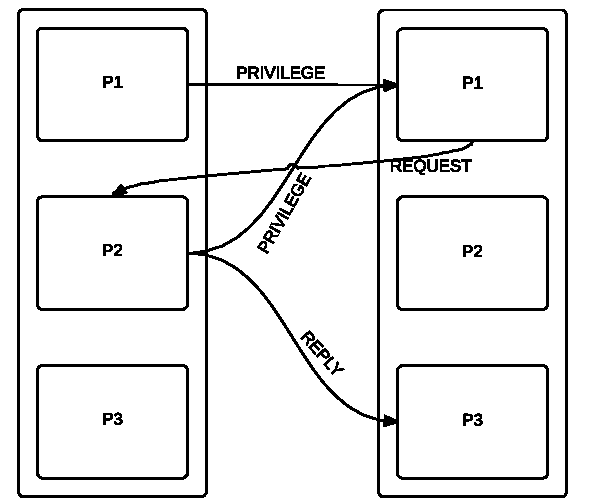
\includegraphics[width=0.55\textwidth]{Skaskam.pdf}
 \caption[Close up of \textit{Hemidactylus} sp.]
   {Two nodes running the \textsc{skam} algorithm, the node to the left holds the privilege. The arrowheads point towards the receiver of the messages.}
\end{center}
\end{figure}


\section{Problem Formulation}
The \textsc{ska} and \textsc{skam} algorithms are claimed to guarantee mutual exclusion, starvation freedom and deadlock freedom. The purpose of this project is to investigate these claims and the additional property of being free from unnecessary delay, using model checking techniques. 

\section{Model of \textsc{ska} and \textsc{skam} in Promela}
Promela is a modelling language with a relatively small set of predefined types and functions. Because of this, a model of the algorithms as specified in the pseudo code (see appendix \ref{sec:ska} and \ref{sec:skam}) must be implemented using the set of instructions available in promela.


\subsection{Nodes}
In the \textsc{ska} algorithm, every node has two processes which have shared variables. This sharing style requires different levels of variable access, i.e. variables that can be accessed by several processes (meaning it is not local), but not by all processes (meaning it is not global). Since only global and local variables exist in promela, the model uses global variables for these shared variables. The global variables are perceived as to belong to a node, and must only be accessed by processes within that node. To ensure this, every node has a node identifier, and this identifier is passed as an argument to each process. 

The convention is that for every shared variable, an array of those variables are created - one for each node. The $i$:th array cell belongs to node $i$, and is the only cell in the array that processes of node $i$ may access.

As an example, consider the boolean variable \texttt{requesting} belonging to node $i$, which must be accessible both by function P1(i) and P2(i). In promela, an array \texttt{requesting[N]} is created, and the processes may only access the cell \texttt{requesting[i]}.

\subsection{Queue}
A queue data structure could be implemented in several ways in promela, with approaches being more or less suited for a certain application. We note that in the \textsc{ska} algorithm, the key features of the queue is first that values are read \emph{first-in first-out} (FIFO) and second the ability to determine whether a certain value is already in the queue or not.

The promela channel data type \texttt{chan}¸is a \textsc{fifo} data structure, but it provides no means of determining if a value is already in the queue or not. To surmount this problem, a new \emph{Queue} data structure is defined;

\begin{lstlisting}
typedef Queue {
  chan ch = [N] of {short};
  bool inQ[N];
}
\end{lstlisting}

This implementation draws upon the fact that a queue in this setting, needs at most store N values, since values may only be added if they are not already in the queue, and the range of numbers that are to be stored are the node identifiers ranging from 0 to N-1.

To add a new value $n$ to the queue, it must first be checked that the value is not already in the queue (i.e. \texttt{inQ[n]} is false). Then the value can be added to the channel \texttt{ch}, and \texttt{inQ[n]} is set to true as to reflect this fact.

To remove the top value from the queue, the opposite is done. The value $n$ is read from the channel \texttt{ch}, and \texttt{inQ[n]} is set to false, indicating that the value $n$ is not in the queue.

\subsection{Messages}
Messages in promela can be sent using the built-in channel datatype (\texttt{chan}). There are different types of messages being sent, \texttt{PRIVILEGE} and \texttt{REQUEST}. To model this, new datatypes were defined as follows;

\begin{lstlisting}
typedef REQUEST{
  chan ch = [N] of {byte, byte};
}

typedef \texttt{PRIVILEGE}{
  chan ch = [N] of {Queue, Array};
}
\end{lstlisting}


In the model, a \texttt{REQUEST} type is created for each node. When a node $i$ requests the privilege with a request identifier $n$, it will write the values $(i,n)$ to the \texttt{REQUEST} channel of each process other than its own. As only one process has the privilege at any time, only one instance of \texttt{PRIVILEGE} needs be created. When a node $i$ wants to send the privilege to another node $j$, node $i$ will write its current queue and its current LN-array to the \texttt{PRIVILEGE} channel.

Since the \texttt{PRIVILEGE} channel can be read by any node, there need be a way to determine which process is to read this channel. This is solved by a global array \texttt{havePrivilege[N]}, that is set to false for all indices except of that belonging to the current holder of the privilege. When the process $i$ above has sent its message on the channel, it will set \texttt (havePrivilege[i]) to false and \texttt (havePrivilege[j]) to true. This indicates to process $j$ that it can read the \texttt{PRIVILEGE} channel.

Note also that it is the changing of the values of havePrivilege that represent the privilege being passed from one process to another, the message channel \texttt{PRIVILEGE} is merely used to pass data structures from one node to another.

The \texttt{REPLY} messages used in the \textsc{skam} algorithm are implemented as a standard channel, writing and reading to the channel correspond to sending and receiving respectively, and the actual values are of no importance.

\subsection{Event Handling}
The process P2 (and in \textsc{skam} also P3) is to be run when a message is received. This indicates a type of event handler, which do not exist in promela. To overcome this problem, we first note that the strength in using a event handler is that it does not rely on \emph{busy waiting}, i.e. a loop that continuously checks whether a certain predicate is true before it continues.

In a classic programming language such a C, busy waiting requires much processing power. In promela on the other hand, an if-statement or a loop for which no predicate is true must always wait until the predicate is true without using busy waiting. This means that busy waiting in promela is not at all ``busy'', and therefore  process P2 can be implemented as a loop with the predicate \texttt{nempty(REQUESTING[i])}.

It is easy to see that the loop will be run once for each message received, and since Spin does not always execute the loop as soon as it is possible, arbitrarily long ``time'' may pass until a \texttt{REQUEST} is actually processed. On the other hand, messages can only be received in the order they are sent whereas in reality a message can be delayed without affecting other messages. 

To solve this issue, the loop can be extended with the non-deterministic choice of reading a message and write it back to the end of the queue, in effect delaying the message. Introducing this choice greatly increase the size of the resulting transition system, and is unlikely to bring the model closer to the original algorithm; re-ordering the queue will merely generate new permutations of its contents, but these permutations would have been checked anyway under a full state space search.


\section{Properties as LTL-Formulae}
Due to the request identifier numbers, the \textsc{ska} algorithm has the disadvantage of unboundedness, meaning that the state space of the model is infinite. There are techniques to overcome these problem, for example to only check the validity of properties within a finite portion of the infinite transition system. Another solution is to model an abstraction of the algorithm, in order to bound the state space (using the fact that the actual \texttt{REQUEST} number is not interesting, only whether it is smaller than some other value or not).

In this paper, the former approach was used to bound the searched portion of the transition system.

\subsection{Deadlock Freedom}
With the spin model checker, deadlocked states are considered to be erroneous states and are included in a standard set of checks run by spin. Thus no extra effort is required to determine the absence of such states, as it will be done automatically unless the model checker is not told to ignore invalid end states. Deadlock freedom can also be shown explicitly for the \textsc{skam} model by checking the LTL-formula

\texttt{[]!timeout}.

\texttt{timeout} is a predefined global read-only name in the promela language, and is true only if no active process is able to proceed.

The corresponding LTL-formula for the \textsc{ska} model simulating two nodes is

\texttt{!timeout U (RN[0].ind[0] > 2 || RN[1].ind[1] > 2)}.

Here \texttt{RN[0].ind[0]} denotes the value of \texttt{RN[0]} in the node with node identifier 0. This formula says that no deadlocks can occur, while the \texttt{REQUEST} numbers of all processes is less than 2. This means that the searched portion of the state space are only those states where all request numbers are lower than 2.

\subsection{Starvation Freedom}
Starvation freedom is the property that no node is consistently overrun by the other processes, i.e. every process will get its turn eventually. This is a liveness property, and needs some degree of fairness to be checked for situations that are reasonable. For example, a node that never requests to enter the critical section will never enter its critical section. Using fairness properties, this kind of irrelevant examples can be excluded. Fairness assumptions can easily be expressed in LTL, in particular it can be expressed that if a process $n_i$ wants to enter its critical section continuously (that is weak fairness), it will always be able to eventually:

 \texttt{<>[]requesting[i] -> []<>havePrivilege[i]}.

The corresponding LTL formula for the \textsc{ska} model simulating two processes is

 \texttt{(requesting[i] -> <>(havePrivilege[i])) U (RN[0].ind[0] > 2 || RN[1].ind[1] > 2)}.

This formula says that if the node with node identifier i requests the privilege, it will eventually get the privilege, while the \texttt{REQUEST} numbers of all processes is less than 2. It is worth noting that expressed in this way, the property is no longer a liveness property but a safety property, and must be checked accordingly.

\subsection{Mutual Exclusion}
Mutual exclusion is the property that at most one node can be executing critical code at the same time. In promela, LTL formula can use built-in \emph{labels} to check properties such as

\texttt{[]!(P1[0]@critSection \&\& P1[1]@critSection)}.

Another way to check for mutual exclusion is to add a shared variable, which is increased by one each time a process enters the critical section, and decreased by one each time it leaves the critical section. The LTL formula to be checked is then

\texttt{[]counter < 2}.

The corresponding LTL formula for the \textsc{ska} model simulating two processes is

\texttt{(counter < 2) U (RN[0].ind[0] > 2 || RN[1].ind[1] > 2)}.

\subsection{Freedom of Unnecessary Delay}
\label{sec:delay}

This describes the property that a process that wishes to enter its critical section must not be delayed unless another process is already in the critical section. In contrast to the terms \emph{Starvation freedom} and \emph{deadlock} that are well-defined term, it is unclear what is to be considered unnecessary delay.

With a rigid definition of ``Unnecessary'', this property is trivially false - a token-based algorithm must at least wait for the token (i.e. the privilege).

On the other hand, a too tolerant definition would make the property trivially true - if a process needs to wait at some point, then surely it is necessary to wait.

Let freedom of \emph{unnecessary delay} imply that when a node holds the privilege, it can enter the critical section without any additional communication with other nodes.

Promela provides the keyword \texttt{dstep}, which can be used to check this property. A block of code written within a \texttt{dstep} block must be executed deterministically; if the process must wait for a message to be received or for a condition to become true, the code is \emph{blocked}. In spin, a block within a \texttt{dstep} is perceived as an error. By enclosing the code following the point where the \texttt{PRIVILEGE} message is received until the end of the critical section within a \texttt{dstep}-block, this property can in effect be checked along side another property, for example while checking for deadlock freedom.

\section{Results}
Exhaustive checking of a property can be very heavy on computation power and memory. To reduce the amount of work needed for testing abstractions and simplifications are used when modelling, and the state space can be reduced by bounding some variables (number of processes, max value of a variable). Still, the amount of memory needed to check a property can soon become infeasible.

The spin model checker also provides a set of tools and techniques that are helpful when checking properties and models of various kinds. To this extent, several modes of compression exist that can reduce the amount of memory needed, but comes with the cost of time. Another technique is to use bitstate hashing of states. Bitstate hashing can reduce the needed memory even more than using compression and without exhibiting the same increase in execution time. The downside is that the results are only an approximation, as the full state space is not guaranteed to be searched.

It is also worth noting that spin uses different techniques when checking for liveness properties than when it checks for safety properties. When checking for safety properties, a finite counter-example is found that does not satisfy the claim, whereas for liveness properties a cycle must be found that does not satisfy the property (optionally under fairness assumptions).

The tests were performed on a system with a dual core processor (2.0 gHz) and with a modest amount of 0.9 \textsc{gb} of \textsc{ram} dedicated to model checking.

\begin{table}

\caption{A summary of the results found for the \textsc{ska} algorithm.}
    \begin{tabular}{l|ll}
    
        ~                              & 2 Processes & 3 Processes             \\ \hline
        Mutual exclusion               & True        & True                    \\ 
        Deadlock freedom               & True        & True                    \\ 
        Starvation freedom             & True        & True (bitstate hashing) \\ 
        freedom from unnecessary delay & True        & True                    \\

    \end{tabular}
\label{tab:skaResults}
\end{table}


\begin{table}[]
\caption{A summary of the results found for the \textsc{skam} algorithm.}

    \begin{tabular}{l|ll}
    
        ~                              & 2 Processes & 3 Processes             \\ \hline
        Mutual exclusion               & True        & -                    \\ 
        Deadlock freedom               & True        & -                    \\ 
        Starvation freedom             & True        & - \\ 
        freedom from unnecessary delay & True (with exception)       & -                    \\

    \end{tabular}
\label{tab:skamResults}
\end{table}

\subsection{Deadlock Freedom}
\label{sec:deadlock}
\begin{figure}[]
\begin{center}
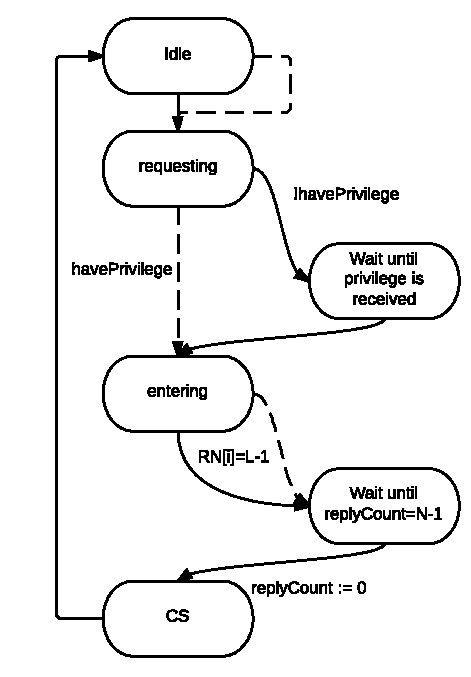
\includegraphics[width=0.5\textwidth]{Deadlock.pdf}
 \caption[Close up of \textit{Hemidactylus} sp.]
   {The behaviour of node $P1_n$ when a deadlock occurs. A continuous line marks a transition in the first iteration, a dashed line a transition in the second iteration. The example begins in the state \emph{idle}.}
\end{center}
\end{figure}

The \textsc{skam} algorithm was shown not to be free from deadlocks, but the deadlock is directly related to the modifications extending \textsc{ska} to \textsc{skam}, and are therefore not present in the \textsc{ska} algorithm.

The problem can occur when a process $P1_n$ requests the \texttt{PRIVILEGE} for the L:th time; after receiving the \texttt{PRIVILEGE} process must wait additionally until the other processes have sent \texttt{REPLY}messages. The indicator of having received replies is a counter \texttt{replyCount}, which is set again to zero when the replies have been received.

The deadlock can occur in the iteration after the Lth, if none of the other processes have requested. If this happens, the process $P1_n$ can attempt to enter the critical section again, and does not need to increase increase its current \texttt{REQUEST} number. As the \texttt{REQUEST} number is unchanged, the process must again wait for the \texttt{REPLY} messages of the other processes, but these have already been sent and received. This marks a deadlock state, where the process holding the \texttt{PRIVILEGE} is waiting infinitely, and no other process can get the privilege. 

This problem can be solved rather simply, by adding a local variable \texttt{nreceived} to the process P1. The variable is set to 0 whenever a \texttt{REQUEST} is made, but said to 1 when all replies have been received. When the process P1 iterates again after its L:th request, it will only wait for replies if the indicator \texttt{nreceived} is not set.

\begin{figure}[]
\begin{center}
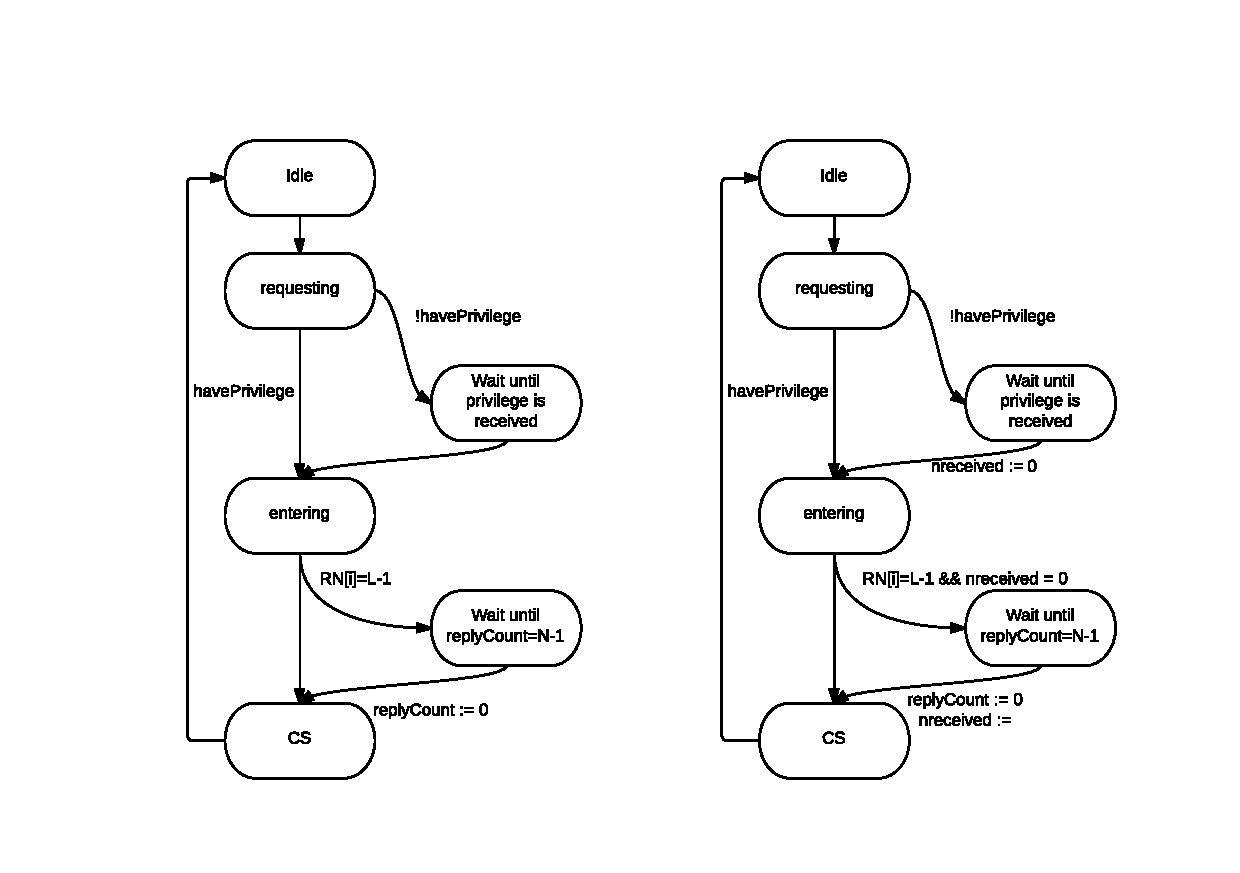
\includegraphics[width=\textwidth]{diagramboth.pdf}
 \caption
   {Simplified flow chart of the \textsc{skam} algorithm (left). Flow chart after extending the model with a variable \texttt{nreceived}}
\end{center}
\end{figure}

Using this small extension the model was shown to be free from deadlocks. All further model checking results are based on the deadlock-free model. Note that it has been assumed that a nodes execute infinitely often (at least the node holding the privilege); without this non-termination assumption, a deadlock might also occur if the process holding the privilege receives a request when still in the critical section, but after checking whether another process is requesting. In this case, if the privilege-holder doesn't request again, the system i sin a deadlock\cite{OgataSAL}\cite{OgataMaude}.

Deadlock freedom was checked successfully for the \textsc{ska} algorithm with two nodes, and with three nodes when checked within a bounded region. It also holds on the textsc{skam} algorithm (after performing the above corrections) with two nodes.

\subsection{Mutual Exclusion}
The tests show that the \textsc{ska} algorithm satisfies mutual exclusion with two nodes and three nodes (within a bounded region of the transition system). The property holds for the \textsc{skam} algorithm, running two nodes.

\subsection{Starvation freedom}
The tests show that the \textsc{ska} algorithm satisfies mutual exclusion with two nodes. Using bitstate hashing, no counterexamples could be found to the claim when running with three nodes.

The property holds for the \textsc{skam} algorithm, running two nodes.

\subsection{Freedom of Unnecessary Delay}
As defined in \ref{sec:delay}, freedom of unnecessary delay implies that a node holding the \texttt{PRIVILEGE} may enter the critical section without any additional communication with other nodes. This property does not hold for the \textsc{skam} algorithm, since every L:th round the node holding the privilege must first wait for \texttt{REPLY} messages from the other nodes.

The results show that the \textsc{ska} algorithm satisfies this property, when running two nodes or three nodes (within a bounded region of the transition system).

The \textsc{skam} algorithm satisfies this property with two whenever the \texttt{REQUEST} identifier of a node is not L-1, checked when running two nodes.

\section{Discussion}
\subsection{The Number of Nodes}
To check the claimed properties, models were checked with two nodes running in parallel, and three nodes when possible. A valid question to ask is whether the results can be said to be more general, that is if they extend to models running four or more processes in parallel.

It is in fact so that running processes with only two parallel nodes cannot exhibit the same behaviour as three nodes could. This is because there are at any state two ``kinds'' of nodes running - the one currently holding the privilege, and the ones that do not. Running with two nodes, some cases cannot occur. For example, when the process P2 receives a request from the other node, havePrivilege[i] will always be true, since if it was false the privilege must belong to the requestee which is a contradiction to the fact that it is currently requesting.

Having seen that two nodes are not enough to fully check the validity of the claims, it is likely that three nodes are. For example, If a node sends a request, it will be received and processes by nodes of both ``kinds''. The differences caused by adding additional nodes are mainly a larger set of variables, larger queues and more permutations of state changes, making model checking much more difficult, but without adding any new \emph{types} of behaviour.

The same arguments can be applied to some fixed-value parameters, such as L in the \textsc{skam} algorithm. There are two different behaviours that can be observed, depending on the value of L; either a request is sent with a value less than L and the algorithm behaves as it does in \textsc{ska}, or a request is sent with the value L meaning values are set to zero and \texttt{REPLY} messages are sent and received.

During testing, a value of $L=2$ was used, but $L=1$ would exhibit the same behaviours with a smaller transition system. 

\subsection{The Validity of Results}
As mentioned above, to formally show that the algorithms truly satisfy the properties, it need be shown for three nodes running in parallel.  As seen in the summaries in table \ref{tab:skaResults} and \ref{tab:skamResults} the properties were shown for to hold for both algorithms with two nodes (after correction of the deadlock, as explained in \ref{sec:deadlock}.

For the \textsc{skam} algorithm, results were not obtainable due to the large state space. The results are inconclusive, as the properties could not be validated nor disproved. 

For the \textsc{ska} algorithm it was shown that the safety properties, mutual exclusion, starvation freedom and freedom of unnecessary delay hold. Starvation freedom was checked using bitstate hashing, which is merely an approximation method. With this said, though it cannot with full certainty be said that starvation freedom holds, this is a strong indication thereof.


\section{references}
\begin{thebibliography}{4}
\bibitem{Suzuki} Suzuki, I., Kasami, T.: A Distributed Mutual Exclusion Algorithm. In: 
ACM Transactions on Computer Systems, Vol. 3, No. 4, November 1985, Pages 344-349.

\bibitem{OgataSAL}Ogata, K., Futatsugi, K.: Analysis of the Suzuki-Kasami Algorithm with SAL Model Checkers. In: 
Proceedings of the 2005 The Fifth International Conference on Computer and Information Technology (CIT 05)

\bibitem{OgataMaude} Ogata, K., Futatsugi, K.: Analysis of the Suzuki-Kasami Algorithm with the Maude Model Checker. In: 
Proceedings of the 12th Asia-Pacific Software Engineering Conference (APSEC 05)




\end{thebibliography}

\newpage
\appendix
\section{Appendix A}
\label{sec:ska}

\begin{lstlisting}[label=some-code,caption=Suzuki and Kasami's algorithm,mathescape]
const I: Integer;		(* the identifier of this node *)
	var HavePrivilege, Requesting:		bool;
	j, n:	 	integer;
	Q: 		queue of integer;
	RN, LN:	array[l . . N] of integer;

	(* The initial values of the variables are:
	HavePrivilege= true in node 1, false in all other nodes;
	Requesting = false; Q = empty;
	RN[j] = -1, j = 1,2, . . . , N;  	LN[j] = -1, j = 1,2,. . . , N; *)

	procedure P1;
	begin
		Requesting := true;
		if not HavePrivilege then
		begin
			RN[I] := RN[I] + 1;
			for all j in {1, 2, . . . , N} - {I} do
				Send REQUEST(I, RN[I]) to node j;
			Wait until PRIVILEGE(Q, LN) is received;
			HavePrivilege:= true
		end,
	
		Critical Section;

		LN[I] := RN[I];
		for all j in {1, 2, . . . , N} - {I} do
			if not in(Q, j) and (RN[jJ = LN[j] + 1) then
				Q := append(Q, j);
		if Q $\neq$ empty then
		begin
			HavePrivilege := false;
			Send PRIVILEGE(tail(Q), LN) to node head(Q)
		end;
		Requesting := false
	end,

	procedure P2; (* REQUEST(j,n) is received; P2 is indivisible *)
	begin
		RN[j] := max(RN[j],n);
		if HavePrivilege and not Requesting and (RN[j] = LN[j] + 1) then
		begin
			HavePrivilege:= false;
			Send PRIVILEGE(Q, LN) to node j
		end
	end,

\end{lstlisting}
\newpage
\section{Appendix B}
\label{sec:skam}

\begin{lstlisting}[label=some-code,caption=Suzuki and Kasami's modified algorithm,mathescape]
const I: integer; (* the identifier of this node *)
	(* Only additional variables shown *)
	ReplyCount :integer;
	RequestCount: array(1 . . N] of integer;
	(* The initial values of the variables are:
		ReplyCount = 0;
		RequestCount[j] = 0, j = 1, 2, . . . , N; *)

	procedure P1;
	begin
		Requesting := true;
		if not HavePrivilege then
		begin
			RN[I] := RN[I] + 1 mod L
			forall j in {1,2,...,N}-{I} do
				Send REQUEST(I, RN[I]) to node j;
	 		Wait until PRIVILEGE(Q, LN) is received;
			HavePrivilege := true
		end;

		Critical Section;
		LN[I] := RN[I];
		if RN[I] = L - 1 then (* end of a round of node I *)
		begin
			Wait until ReplyCount = N - 1;
			ReplyCount := 0
		end;
		for all j in {1, 2, . . . , N} - {I} do
			if not in(Q, j) and (RN[jJ = LN[j] + 1 mod L) then Q := append(Q, j);
		if Q $\neq$ empty then
		begin
			HavePrivilege := false;
			Send PRIVILEGE(taiI(Q), LN) to node head(Q)
		end,
		Requesting := false
	end:

	procedure P2; (* REQUEST(j, n) is received; P2 is indivisible *)
	begin
		RequestCount[ j] := RequestCount[ j] + 1;
		if Request Count[j] = L then
		begin
			Send REPLY to node j;
			RequestCount[ j] := 0
		end,

		if RequestCount[ j] = 1 then RN] j] := n (* beginning of a new round of node j *)
		else RN[j] := max(RN[j], n);
	
		if HavePrivilege and not Requesting and (RN[j] = LN[jJ + 1 mod L) then
		begin
			HavePrivilege := false;
			Send PRIVILEGE(Q, LN) to node j
		end
	end;



	procedure P3; (* REPLY is received *)
	begin
		ReplyCount := ReplyCount + 1
	end;

\end{lstlisting}


\end{document}

